\section{Sở GD\&ĐT  Lào Cai --Lần 1 NH: 2025--2026}
\caulc
%======Câu_1-phần I======%
\begin{ex}%[2H2H2-4]
	Trong không gian $(Oxyz)$, cho hai điểm $A(1;1;-3)$ và $B(2;-1;-1)$. Độ dài đoạn $AB$ bằng
\choice
	{\True $3$}
	{$4$}
	{$3\sqrt{2}$}
	{$4\sqrt{2}$}
\loigiai{Ta có $\vec{AB}=(2-1;-1-1;-1-(-3))=(1;-2;2)$.\\
		Độ dài đoạn thẳng $AB$ là $AB=\sqrt{1^2+(-2)^2+2^2}=\sqrt{9}=3$.\\
	}
\end{ex}

%======Câu_2-phần I======%
\begin{ex}%[2D4H3-4]
	Khi cắt một vật thể bởi mặt phẳng vuông góc với trục $Ox$ tại điểm có hoành độ $x$ với mặt cắt là hình vuông có độ dài các cạnh là $\sqrt{3-x^2}$ ($-\sqrt{3} \le x \le \sqrt{3}$). Thể tích của vật thể đã cho bằng
\choice
	{$\pi\sqrt{3}$}
	{\True $4\sqrt{3}$}
	{$\sqrt{3}$}
	{$4\pi\sqrt{3}$}
\loigiai{
		Diện tích mặt cắt tại hoành độ $x$ là hình vuông cạnh $a = \sqrt{3-x^2}$ nên ta có 
		$S(x) = \left( \sqrt{3-x^2} \right)^2 = 3-x^2$.
		Thể tích của vật thể đã cho là
		$$V = \displaystyle\int\limits_{-\sqrt{3}}^{\sqrt{3}} S(x) \mathrm{\,d}x = \displaystyle\int\limits_{-\sqrt{3}}^{\sqrt{3}} (3-x^2) \mathrm{\,d}x = \left. \left( 3x - \dfrac{x^3}{3} \right) \right|_{-\sqrt{3}}^{\sqrt{3}} = 4\sqrt{3}.$$
	}
\end{ex}

%======Câu_3-phần I======%
\begin{ex}%[1D1N4-2]
	Tập xác định của hàm số $y=\cot x$ là
\choice
	{$\mathbb{R}\setminus\left\{\dfrac{\pi}{2}+k2\pi,k\in\mathbb{Z}\right\}$}
	{\True $\mathbb{R}\setminus\{k\pi,k\in\mathbb{Z}\}$}
	{$\mathbb{R}\setminus\{k2\pi,k\in\mathbb{Z}\}$}
	{$\mathbb{R}\setminus\left\{\dfrac{\pi}{2}+k\pi,k\in\mathbb{Z}\right\}$}
\loigiai{Hàm số $y=\cot x$ xác định khi $\sin x\ne 0\Leftrightarrow x\ne k\pi,k\in\mathbb{Z}$.\\
		Vậy tập xác định là $D=\mathbb{R}\setminus\{k\pi,k\in\mathbb{Z}\}$.}
\end{ex}

%======Câu_4-phần I======%
\begin{ex}%[1H8H1-3]
	Cho hình lập phương $ABCD.EFGH$. Góc giữa hai đường thẳng $AF$ và $EG$ là
\choice
	{$90^{\circ}$}
	{\True $60^{\circ}$}
	{$0^{\circ}$}
	{$30^{\circ}$}
\loigiai{
		\immini{
			Ta có $EG\parallel AC$ nên $(AF,EG)=(AF,AC)$.\\
			Xét tam giác $AFC$ có $AF=FC=CA$ (đều là đường chéo của các mặt hình lập phương bằng nhau).\\
			Do đó tam giác $AFC$ là tam giác đều, suy ra $\widehat{FAC}=60^\circ$.\\
			Vậy góc giữa hai đường thẳng là $60^\circ$.
		}{
			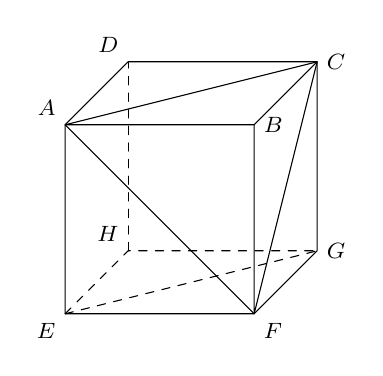
\begin{tikzpicture}[scale=0.8, font=\footnotesize, line join=round, line cap=round, >=stealth]
				% Tọa độ các đỉnh
				\coordinate (E) at (0,0);
				\coordinate (F) at (3,0);
				\coordinate (G) at (4,1);
				\coordinate (H) at (1,1);
				\coordinate (A) at (0,3);
				\coordinate (B) at (3,3);
				\coordinate (C) at (4,4);
				\coordinate (D) at (1,4);
				\draw (A) -- (B) -- (C) -- (D) -- cycle;
				\draw (F)--(C)--(A) -- (E) -- (F) -- (B);
				\draw (F) -- (G) -- (C);
				\draw[dashed] (E) -- (H) -- (G);
				\draw[dashed] (H) -- (D);
				\draw (A) -- (F);
				\draw[dashed] (E) -- (G);
				\node[above left] at (A) {$A$};
				\node[right] at (B) {$B$};
				\node[right] at (C) {$C$};
				\node[above left] at (D) {$D$};
				\node[below left] at (E) {$E$};
				\node[below right] at (F) {$F$};
				\node[right] at (G) {$G$};
				\node[above left] at (H) {$H$};
			\end{tikzpicture}
		}
	}
\end{ex}

%======Câu_5-phần I======%
\begin{ex}%[1D2N3-4]
	Cho cấp số nhân $(u_n)$ với $u_1=3$ và công bội $q=4$. Giá trị của $u_2$ bằng
\choice
	{$5$}
	{$\dfrac{4}{3}$}
	{\True $12$}
	{$\dfrac{3}{4}$}
\loigiai{Công thức tính số hạng của cấp số nhân là $u_n=u_1\cdot q^{n-1}$.\\
		Với $n=2$, ta có $u_2=u_1\cdot q=3\cdot 4=12$.}
\end{ex}

%======Câu_6-phần I======%
\begin{ex}%[2D1H4-1]
	\immini{Cho hàm số $y=f(x)=\dfrac{ax^2+bx+c}{mx+n}$ có đồ thị như hình vẽ bên dưới. Đường tiệm cận xiên của đồ thị hàm số đã cho có phương trình là
\choice
	{$y=x-1$}
	{$y=3x+1$}
	{$y=x-2$}
	{\True $y=x+3$}
}
	{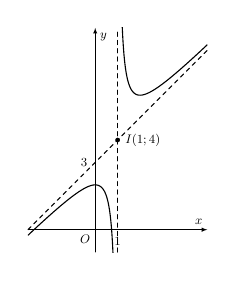
\begin{tikzpicture}[scale=0.5, font=\footnotesize, line join=round, line cap=round, >=stealth]
			\begin{axis}[
				axis lines = middle,
				xlabel = $x$,
				ylabel = $y$,
				xmin = -3, xmax = 5,
				ymin = -1, ymax = 9,
				xtick = {1},
				ytick = {3},
				%extra x ticks={0},
				%extra y ticks={0},
				tick style={draw=none},
				unit vector ratio={1 1}, % Giữ tỉ lệ trục 1:1
				restrict y to domain=-2:12,
				samples=200,
				axis line style={-latex},
				font=\small
				]
				
				% Vẽ tiệm cận đứng x = 1
				\draw[dashed, thick] (axis cs:1,-1) -- (axis cs:1,9);
				%\node[below right] at (axis cs:1,0) {1};
				
				% Vẽ tiệm cận xiên y = x + 3
				\addplot[dashed, thick, domain=-3:5] {x+3};
				\node[left] at (axis cs:0,3) {};
				
				% Vẽ đồ thị hàm số (nhánh trái)
				\addplot[thick, color=black, domain=-3:0.85] {(x^2 + 2*x - 2)/(x - 1)};
				
				% Vẽ đồ thị hàm số (nhánh phải)
				\addplot[thick, color=black, domain=1.15:5] {(x^2 + 2*x - 2)/(x - 1)};
				
				% Đánh dấu tâm đối xứng I(1,4)
				\filldraw (axis cs:1,4) circle (1.5pt) node[right, xshift=2pt] {$I(1;4)$};
				
				% Gốc tọa độ
				\node[below left] at (axis cs:0,0) {$O$};
				
			\end{axis}
	\end{tikzpicture}}
	\loigiai{
		Dựa vào hình vẽ, ta thấy đường tiệm cận xiên đi qua điểm $I(1;4)$ và cắt trục tung tại điểm có tung độ bằng $3$, tức là điểm $(0;3)$.\\
		Phương trình đường thẳng có dạng $y=ax+b$.\\
		Thay tọa độ hai điểm vào ta có hệ: $\begin{cases} a\cdot 0+b=3 \\ a\cdot 1+b=4 \end{cases} \Leftrightarrow \begin{cases} b=3 \\ a=1 \end{cases}$.\\
		Vậy phương trình đường tiệm cận xiên là $y=x+3$.
	}
\end{ex}

%======Câu_7-phần I======%
\begin{ex}%[1D6H4-3]
	Tập nghiệm của bất phương trình $3^{x-1}\ge 9$ là
\choice
	{$[2;+\infty)$}
	{$(-\infty;2)$}
	{\True $[3;+\infty)$}
	{$(-\infty;3]$}
\loigiai{
		Ta có $3^{x-1}\ge 9 \Leftrightarrow 3^{x-1}\ge 3^2$.\\
		Vì cơ số $3>1$ nên bất phương trình tương đương với $x-1\ge 2 \Leftrightarrow x\ge 3$.\\
		Vậy tập nghiệm của bất phương trình là $S=[3;+\infty)$.
	}
\end{ex}

%======Câu_8-phần I======%
\begin{ex}%[2H2N2-3]
	Trong không gian $Oxyz$, cho hai véc-tơ $\vec{a}=(1;2;-1)$ và $\vec{b}=(2;-1;3)$. Tọa độ của véc-tơ $4\vec{a}-\vec{b}$ là
\choice
	{\True $(2;9;-7)$}
	{$(2;9;7)$}
	{$(-2;9;7)$}
	{$(-2;-9;7)$}
\loigiai{
		Ta có $4\vec{a}=4(1;2;-1)=(4;8;-4)$.\\
		Khi đó $4\vec{a}-\vec{b}=(4-2;8-(-1);-4-3)=(2;9;-7)$.\\
		Vậy tọa độ véc-tơ cần tìm là $(2;9;-7)$.
	}
\end{ex}

%======Câu_9-phần I======%
\begin{ex}%[2D3N2-2]
	Khảo sát thời gian tự học bài ở nhà của học sinh khối 9 ở trường X, ta thu được bảng sau:
	\begin{center}
		\begin{tabular}{|c|c|c|c|c|c|}
			\hline
			Thời gian (phút) & $[0;30)$ & $[30;60)$ & $[60;90)$ & $[90;120)$ & $[120;150)$ \\ \hline
			Số học sinh & $9$ & $10$ & $9$ & $15$ & $7$ \\ \hline
		\end{tabular}
	\end{center}
	Phương sai của mẫu số liệu ghép nhóm là
\choice
	{$1602$}
	{\True $1601{,}64$}
	{$1601{,}9$}
	{$1603$}
\loigiai{
		Giá trị đại diện của các nhóm lần lượt là: $x_1=15$, $x_2=45$, $x_3=75$, $x_4=105$, $x_5=135$.\\
		Tổng số học sinh $n=9+10+9+15+7=50$.\\
		Số trung bình $\bar{x}=\dfrac{9\cdot 15+10\cdot 45+9\cdot 75+15\cdot 105+7\cdot 135}{50}=75{,}6$.\\
		Phương sai $s^2=\dfrac{1}{50}[9\cdot 15^2+10\cdot 45^2+9\cdot 75^2+15\cdot 105^2+7\cdot 135^2] - 75{,}6^2 = 1601{,}64$.
	}
\end{ex}

%======Câu_10-phần I======%
\begin{ex}%[2D1N2-2]
	\immini{Cho hàm số $f(x)$ có bảng biến thiên như hình vẽ. 
		Hàm số đã cho đạt cực đại tại
\choice
	{$x=2$}
	{\True $x=-1$}
	{$x=-2$}
	{$x=1$}
}{
		
\begin{tikzpicture}[>=stealth,scale=.8]
			\tkzTabInit[lgt=1.2,espcl=2.5,deltacl=0.5]{$x$/.6,$f'(x)$/.6,$f(x)$/1.8}{$-\infty$,$-1$,$2$,$+\infty$}
			\tkzTabLine{,$+$,0,$-$,0,$+$,}
			\tkzTabVar{-/ $-\infty$,+/ $1$,-/ $-2$,+/ $+\infty$}
	\end{tikzpicture}}
	
	\loigiai{Dựa vào bảng biến thiên, ta thấy đạo hàm $f'(x)$ đổi dấu từ dương sang âm khi đi qua $x=-1$.\\
		Do đó, hàm số đã cho đạt cực đại tại điểm $x=-1$.}
\end{ex}

%======Câu_11-phần I======%
\begin{ex}%[2D4N1-4]
	Nguyên hàm của hàm số $y=5^x$ là
\choice
	{$5^x\cdot\ln5+C$}
	{$x\cdot5^{x-1}+C$}
	{\True $\dfrac{5^x}{\ln5}+C$}
	{$\dfrac{5^{x+1}}{x+1}+C$}
\loigiai{
		Ta có $\displaystyle\int 5^x \mathrm{d}x = \dfrac{5^x}{\ln 5}+C$.}
\end{ex}

%======Câu_12-phần I======%
\begin{ex}%[2H2N1-1]
	Cho hình lập phương $ABCD.A'B'C'D'$. Khi đó $\overrightarrow{AD'}$ bằng véc-tơ nào sau đây?
\choice
	{$\overrightarrow{BC}$}
	{\True $\overrightarrow{BC'}$}
	{$\overrightarrow{B'C'}$}
	{$\overrightarrow{BB'}$}
\loigiai{
		\immini{Xét tứ giác $ABC'D'$, ta có $AD' \parallel BC'$ và $AD' = BC'$ \\
			Vậy $\overrightarrow{AD'}=\overrightarrow{BC'}$.}
		{
			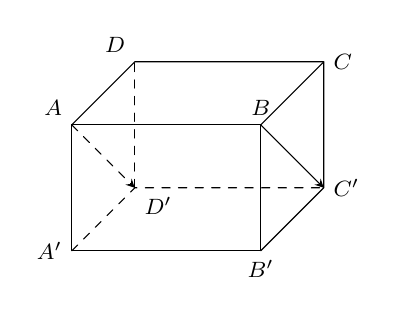
\begin{tikzpicture}[scale=0.8, font=\footnotesize, line join=round, line cap=round, >=stealth]
				% Tọa độ các đỉnh
				\coordinate (A) at (0,2); \coordinate (B) at (3,2);
				\coordinate (C) at (4,3); \coordinate (D) at (1,3);
				\coordinate (A1) at (0,0); \coordinate (B1) at (3,0);
				\coordinate (C1) at (4,1); \coordinate (D1) at (1,1);
				
				% Vẽ các cạnh thấy được
				\draw (A) -- (B) -- (B1) -- (A1) -- cycle;
				\draw (B) -- (C) -- (C1) -- (B1);
				\draw (C) -- (D) -- (A);
				
				% Vẽ các cạnh khuất
				\draw[dashed] (A1) -- (D1) -- (C1);
				\draw[dashed] (D1) -- (D);
				
				% Vẽ các véc-tơ minh họa
				\draw[dashed, ->] (A) -- (D1);
				\draw[->] (B) -- (C1);
				
				% Gán nhãn các đỉnh
				\node[above left] at (A) {$A$}; \node[above] at (B) {$B$};
				\node[right] at (C) {$C$}; \node[above left] at (D) {$D$};
				\node[left] at (A1) {$A'$}; \node[below] at (B1) {$B'$};
				\node[right] at (C1) {$C'$}; \node[below right] at (D1) {$D'$};
			\end{tikzpicture}
		}
	}
\end{ex}

\cauds
%======Câu_1-phần II======%
\begin{ex}%[2D4V2-3]
Cho hàm số $f(x)=\sin x+\cos x$ và $g(x)=3-2\sin x$.
\choiceTF
	{\True $\displaystyle\int\limits_0^{\tfrac{\pi}{2}}f(x)\,\mathrm{d}x=2$}
	{\True Tập giá trị của hàm số $g(x)=3-2\sin x$ là $T=[1;5]$}
	{$\displaystyle\int g(x)\,\mathrm{d}x=3x-2\cos x+C$}
	{\True Số nghiệm phương trình $\displaystyle \int\limits_0^{\tfrac{\pi}{2}}f(x)\mathrm{d}x=3-2\sin x$ trên đoạn $[0;2\pi]$ là $2$}
\loigiai{
\begin{itemchoice}
	\itemch $\displaystyle\int\limits_0^{\tfrac{\pi}{2}}f(x)\,\mathrm{d}x=\displaystyle\int\limits_{0}^{\tfrac{\pi}{2}} \left(\sin x+\cos x\right) \mathrm{d}x=(-\cos x+\sin x)\Big|_{0}^{\tfrac{\pi}{2}}=\left(-\cos \dfrac{\pi}{2}+\sin\dfrac{\pi}{2}\right)-\left(-\cos 0+\sin 0\right)=2$.
	\itemch Ta có $-1\leq -\sin x \leq 1 \Leftrightarrow -2\leq -2\sin x \leq 2 \Leftrightarrow 3-2\leq 3-2\sin x\leq 3+2 \Leftrightarrow 1 \leq y \leq 5$.\\
	Vậy tập giá trị của hàm số $g(x)=3-2\sin x$ là $T=[1;5]$.
	\itemch Ta có $\displaystyle\int g(x)\,\mathrm{d}x=\displaystyle\int (3-2\sin x)\,\mathrm{d}x=3x+2\cos x+C$.
	\itemch Xét phương trình
			\allowdisplaybreaks
	\begin{eqnarray*}
		&& \displaystyle \int\limits_0^{\tfrac{\pi}{2}}f(x)\mathrm{d}x=3-2\sin x \\ 
	&\Leftrightarrow&3-2\sin x=2\\
	&\Leftrightarrow&\sin x=\dfrac{1}{2}\\
		&\Leftrightarrow&\hoac{& x=\dfrac{\pi}{6}+k2\pi\\&x=\dfrac{5\pi}{6}+k2\pi.}~(k\in\mathbb{Z})
	\end{eqnarray*}
	Vì $x\in [0;2\pi]$ nên tập nghiệm của phương trình trên đoạn $[0;2\pi]$ là $S=\left\{\dfrac{\pi}{6};\dfrac{5\pi}{6}\right\}$.\\
	Vậy số nghiệm phương trình $\displaystyle \int\limits_0^{\tfrac{\pi}{2}}f(x)\mathrm{d}x=3-2\sin x$ trên đoạn $[0;2\pi]$ là $2$.
\end{itemchoice}}
\end{ex}

%======Câu_2-phần II======%
\begin{ex}%[2H2V1-3]
\immini{Cho hình lập phương $ABCD.A'B'C'D'$ có cạnh bằng $a$ (tham khảo hình vẽ).
\choiceTF
	{\True $\overrightarrow{AC}=\overrightarrow{AB}+\overrightarrow{AD}$}
	{\True $\overrightarrow{AC'}=\overrightarrow{AD}+\overrightarrow{AB}+\overrightarrow{AA'}$}
	{\True $(\overrightarrow{AC},\overrightarrow{B'C'})=45^\circ$}
	{$\overrightarrow{AC}\cdot\overrightarrow{B'C'}=\dfrac{\sqrt{2}a^2}{2}$}
}{
\begin{tikzpicture}[scale=0.6,font={\footnotesize},>=stealth]	
	\path
	(0,0) coordinate (D)
	(1.2,1.45) coordinate (A)
	(4,0) coordinate (C)
	($(A)+(C)-(D)$) coordinate (B)
	($(A)+(0,4)$) coordinate (A')
	($(B)+(0,4)$) coordinate (B')
	($(C)+(0,4)$) coordinate (C')
	($(D)+(0,4)$) coordinate (D')
	;
	\draw[dashed] (B)--(A)--(D)  (A)--(A') ;
	\draw (B)--(C)--(D) (B)--(B') (C)--(C') (D)--(D') (A')--(B')--(C')--(D')--(A') ;
	% vẽ điểm
	\foreach \x/\g in {A/160,B/0,C/-90,D/-90,A'/90,B'/90,C'/-30,D'/180}
	\draw[fill=black] (\x) circle (1pt)+(\g:.27)
	node{$\x$};		
	\end{tikzpicture}}
	\loigiai{
	\begin{itemchoice}
	\itemch Vì $ABCD$ là hình vuông nên áp dụng qui tắc hình bình hành ta có $\overrightarrow{AC}=\overrightarrow{AB}+\overrightarrow{AD}$.
	\itemch Áp dụng qui tắc hình hộp ta có $\overrightarrow{AC'}=\overrightarrow{AB}+\overrightarrow{AD}+\overrightarrow{AA'}$.
	\itemch Vì $B'C' \parallel BC$ nên $\left(\overrightarrow{AC},\overrightarrow{B'C'}\right)=\left(\overrightarrow{AC},\overrightarrow{BC}\right)=\left(\overrightarrow{CA},\overrightarrow{CB}\right)=\widehat{ACB}=45^\circ$ ($ABCD$ là hình vuông).
	\itemch $\overrightarrow{AC}\cdot\overrightarrow{B'C'}=\left|\overrightarrow{AC}\right|\cdot\left|\overrightarrow{B'C'}\right|\cos\left(\overrightarrow{AC},\overrightarrow{B'C'}\right)=a\sqrt{2} \cdot a \cdot \cos 45^\circ=a^2$.
\end{itemchoice}}
\end{ex}

%======Câu_3-phần II======%
\begin{ex}%[2D1V5-1]
	\immini{Cho hàm số $y=\dfrac{ax^2+bx+c}{mx+n}$ có đồ thị như hình vẽ bên.
\choiceTF
	{Hàm số nghịch biến trên khoảng $(-1;0)$}
	{\True $m=n$}
	{\True Tâm đối xứng của đồ thị hàm số là $I(-1;2)$}
	{\True Khoảng cách giữa hai điểm cực trị của đồ thị hàm số bằng $2\sqrt{5}$}
}{
		\begin{tikzpicture}[scale=0.5,font={\footnotesize},>=stealth]	
		%%Nhập giới hạn đồ thị và hàm số cần vẽ
		\def \xmin{-6}
		\def \xmax{4}
		\def \ymin{-4}
		\def \ymax{7}
		%%Tự động
		\draw[->] (\xmin,0)--(\xmax,0) node[shift=(90:0.25)] {$x$};
		\draw[->] (0,\ymin)--(0,\ymax) node[shift=(180:0.25)] {$y$};
		\draw (0,0) node [shift=(135:0.25)] {$O$};
		\clip(\xmin-0.1,\ymin-0.1) rectangle (\xmax+0.1,\ymax+0.1);
		%%Vẽ các điểm trên 2 hệ trục
		\draw[samples=350,domain=-6:-1.2,smooth,variable=\x] plot (\x,{(-(\x)^2)/(\x+1)});
		\draw[samples=350,domain=-0.84:3.53,smooth,variable=\x] plot (\x,{(-(\x)^2)/(\x+1)});
		\draw[dashed] (-1,\ymin)--(-1,\ymax) ;
		\draw[dashed,samples=350,domain=\xmin:\xmax,smooth,variable=\x] plot (\x,{-(\x)+1});
		\draw[dashed] 
		(-2,0)node[shift=(-90:0.25)]{$-2$} |- (0,4)node[shift=(0:0.22)]{$4$}
		(-1,2) --(0,2) node[shift=(0:0.22)]{$2$}
		(-1,0) node[shift=(150:0.25)]{$-1$}
		(0,1) node[shift=(0:0.22)]{$1$}
		;
	\end{tikzpicture}}
	\loigiai{
		\begin{itemchoice}
			\itemch Dựa vào đồ thị, hàm số đã cho nghịch biến trên các khoảng $(-\infty;-2)$ và $(0;+\infty)$.
			\itemch Vì $x=-1$ là tiệm cận đứng của đồ thị hàm số $y=\dfrac{ax^2+bx+c}{mx+n}$.\\
			Nên $x=-1$ là nghiệm của phương trình $mx+n=0$.\\
			Khi đó $-m+n=0 \Rightarrow m=n$.
			\itemch Dựa vào đồ thị, ta thấy tiệm cận đứng và tiệm cận xiên của đồ thị hàm số $y=\dfrac{ax^2+bx+c}{mx+n}$ cắt nhau tại $I(-1;2)$.\\
			Do đó đồ thị hàm số $y=\dfrac{ax^2+bx+c}{mx+n}$ có tâm đối xứng là $I(-1;2)$.
			\itemch Dựa vào đồ thị, ta thấy đồ thị hàm số $y=\dfrac{ax^2+bx+c}{mx+n}$ có hai điểm cực trị là $A(-2;4)$ và $O(0;0)$.\\
			Do đó khoảng cách giữa hai điểm cực trị là $OA=\sqrt{(-2)^2+4^2}=2\sqrt{5}$. 
	\end{itemchoice}}
\end{ex}

%======Câu_4-phần II======%
\begin{ex}%[2D4V2-6]
	\immini{Một người chuyển động trên một quãng đường thẳng, mối quan hệ giữa vận tốc và thời gian được minh họa như hình vẽ. Đường cong trong hình vẽ là một phần của parabol có đỉnh tại điểm có vận tốc $22$ m/s.
}{
	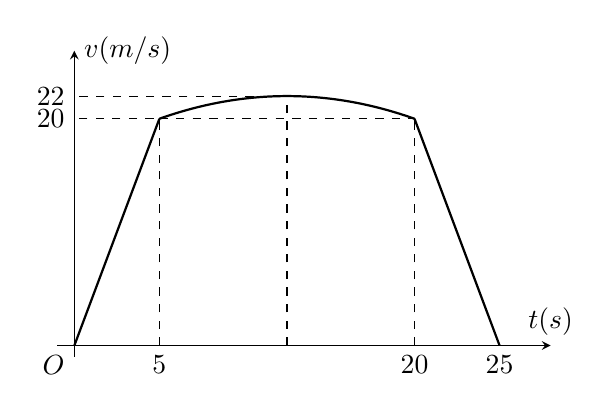
\begin{tikzpicture}[>=stealth, xscale=0.27, yscale=0.18,scale=0.8]
		% Trục tọa độ
		\draw[->] (-1,0) -- (28,0) node[above] {$t(s)$};
		\draw[->] (0,-1) -- (0,26) node[right] {$v(m/s)$};
		\node[below left] at (0,0) {$O$};
		
		% Các điểm mốc trên trục
		\node[below] at (5,0) {$5$};
		\node[below] at (20,0) {$20$};
		\node[below] at (25,0) {$25$};
		\node[left] at (0,20) {$20$};
		\node[left] at (0,22) {$22$};
		
		% Vẽ đoạn thẳng đầu (0,0) đến (5,20)
		\draw[thick] (0,0) -- (5,20);
		
		% Vẽ cung parabol từ t=5 đến t=20
		% Parabol đi qua (5,20), (20,20) và đỉnh tại trung điểm t=12.5 có v=22
		% Phương trình dạng v = a(t-12.5)^2 + 22. Thay t=5, v=20 => 20 = a(-7.5)^2 + 22 => a = -2/56.25 = -8/225
		\draw[thick, samples=100, domain=5:20] plot (\x, {-8/225*(\x-12.5)^2 + 22});
		
		% Vẽ đoạn thẳng cuối (20,20) đến (25,0)
		\draw[thick] (20,20) -- (25,0);
		
		% Đường dóng
		\draw[dashed] (5,0) -- (5,20) -- (0,20) (5,20)--(20,20);
		\draw[dashed] (20,0) -- (20,20);
		\draw[dashed] (12.5,22) -- (0,22);
		\draw[dashed] (12.5,0) -- (12.5,22);
		\fill (12.5,22) circle (2pt);
		\end{tikzpicture}}
	\choiceTF
	{Trong $5$ giây đầu tiên, người đó chuyển động nhanh dần đều với gia tốc $a=5$ m/s$^2$}
	{Quãng đường đi được trong $5$ giây đầu tiên là $100$ m}
	{\True Quãng đường vật đi được trong $20$ giây đầu tiên là $370$ m}
	{\True Vận tốc trung bình của người đó trên cả hành trình là $16{,}8$ m/s}
	\loigiai{
	\begin{itemchoice}
		\itemch Trong $5$ giây đầu tiên, đồ thị vận tốc là đường thẳng $v_1(t)=kt$ đi qua $A(5;20)$.\\
		Khi đó $20=5k \Rightarrow k=4$.\\
		Suy ra $v_1(t)=4t$ (m/s).\\
		Do đó gia tốc người đó là $a=v_1'(t)=4$ (m/s$^2$).
		\itemch Quãng đường đi được trong $5$ giây đầu tiên là  $S_1=\displaystyle\int\limits_{0}^{5} v_1(t)\,\mathrm{d}t=\displaystyle\int\limits_{0}^{5} 4t\,\mathrm{d}t=50\,(\text{m}).$ 
		\itemch Khi $t\in [5;20]$, đồ thị vận tốc là một parabol có hàm số $v_2(t)=at^2+bt+c$.\\
		Hoành độ đỉnh của parabol là $x_I=\dfrac{-b}{2a}=12{,}5$. Suy ra $25a+b=0$.\hfill$(1)$\\
		Vì parabol đi qua điểm $I(12{,}5;22)$ nên $a\cdot \left(12{,}5\right)^2+b\cdot (12{,}5)+c=22$.\hfill$(2)$\\
		Vì parabol đi qua điểm $A(5;20)$ nên $a\cdot 5^2+b\cdot 5+c=20$.\hfill$(3)$\\
		Từ $(1)$, $(2)$, $(3)$ giải hệ phương trình ta được $a=-\dfrac{8}{225}$; $b=\dfrac{8}{9}$ và $c=\dfrac{148}{9}$.\\
		Vậy quãng đường vật đi được trong $20$ giây đầu tiên là
		\[S_1+\displaystyle\int\limits_{5}^{20} v_2(t)\,\mathrm{d}t=50+\displaystyle\int\limits_{5}^{20} \left(-\dfrac{8}{225}t^2+\dfrac{8}{9}t+\dfrac{148}{9}\right)\,\mathrm{d}t=370\,(\text{m}).\]
		\itemch Khi $t\in[20;25]$, đồ thị vận tốc là đường thẳng $v_2(t)=mt+n$ đi qua $B(20;20)$, $C(25;0)$.\\
		Vì $B(20;20)$ thuộc đồ thị $v_2(t)$ nên $20m+n=20$.\hfill$(4)$\\
		Vì $C(25;0)$ thuộc đồ thị $v_2(t)$ nên $25m+n=0$.\hfill$(5)$\\
		Từ $(4)$, $(5)$ giải hệ phương trình ta được $m=-4$; $n=100$.\\
		Tổng quãng đường người đó đi được trong $25$ giây đầu tiên là $370+\displaystyle\int\limits_{20}^{25} (-4t+100)\,\mathrm{d}t=420\,(\text{m})$.\\
		Vận tốc trung bình của người đó trên cả hành trình là $\dfrac{420}{25}=16{,}8$ (m/s).
	\end{itemchoice}}
\end{ex}

\caukq
%======Câu_1-phần III======%
\begin{ex}%[1H8V6-6]
	Cho hình chóp $S.ABCD$ có đáy $ABCD$ là hình thoi tâm $O$, cạnh bằng $6$ và góc $\widehat{ABC}=60^\circ$. Biết rằng hình chiếu vuông góc của $S$ lên mặt phẳng $(ABCD)$ trùng với trọng tâm $G$ của tam giác $ABC$ và số đo góc nhị diện $[S,AC,G]$ bằng $60^\circ$. Khi đó, khoảng cách giữa hai đường thẳng $SD$ và $AC$ bằng $\dfrac{b}{\sqrt{a}}$ (với $a,b\in\mathbb{Z}$, $a$, $b$ là hai số nguyên tố cùng nhau). Giá trị của $a^2-b^2$ bằng bao nhiêu?
\par\shortans{$280$}
\loigiai{
		\immini{Gọi $O$ là tâm hình thoi $ABCD$. Vì $ABCD$ là hình thoi có $\widehat{ABC}=60^\circ$ nên $\Delta ABC$ đều cạnh $6$.\\
			Suy ra $AC=6$ và đường cao $BO=\dfrac{6\sqrt{3}}{2}=3\sqrt{3}\Rightarrow BD=6\sqrt{3}$.\\
			$G$ là trọng tâm $\Delta ABC$ nên $G\in BO$, $BG=\dfrac{2}{3}BO=2\sqrt{3}$, $GO=\dfrac{1}{3}BO=\sqrt{3}$.\\
			Do $S$ có hình chiếu vuông góc lên $(ABCD)$ là $G$ nên $SG\perp(ABCD)$.\\
			Ta có $AC\perp BD\Rightarrow AC\perp GO$. Lại có $AC\perp SG$ nên $AC\perp(SBD)\Rightarrow AC\perp SO$.\\
			Từ đó, góc nhị diện $[S,AC,G]$ chính là $\widehat{SOG}=60^\circ$.\\
			Trong $\Delta SGO$ vuông tại $G$, ta có $SG=GO\cdot\tan60^\circ=\sqrt{3}\cdot\sqrt{3}=3$.}
		{
			\begin{tikzpicture}[scale=0.7, font=\footnotesize, line join=round, line cap=round, >=stealth]
				\coordinate (B) at (0,0);
				\coordinate (C) at (4,0);
				\coordinate (A) at (1.5, 2);
				\coordinate (D) at (5.5, 2);
				\coordinate (O) at (2.75, 1);
				\coordinate (G) at (1.833, 0.667); 
				\coordinate (S) at (1.833, 4.5);
				\coordinate (H) at ($(S)!0.4!(D)$);
				\draw (B) -- (C) -- (D) -- (S) -- cycle;
				\draw (S) -- (C);
				\draw[dashed] (A) -- (B) (A) -- (D) (S) -- (A) (A) -- (C) (B) -- (D) (S) -- (G) (S) -- (O)--(H);
				\fill (A) circle (1.5pt) node[above left] {$A$};
				\fill (B) circle (1.5pt) node[below left] {$B$};
				\fill (C) circle (1.5pt) node[below right] {$C$};
				\fill (D) circle (1.5pt) node[above right] {$D$};
				\fill (O) circle (1.5pt) node[below] {$O$};
				\fill (G) circle (1.5pt) node[below left] {$G$};
				\fill (S) circle (1.5pt) node[above] {$S$};
				\fill (H) circle (1.5pt) node[above] {$H$};
		\end{tikzpicture}}
		\noindent Ta có $AC\perp(SBD)$ tại $O$. Trong mặt phẳng $(SBD)$, kẻ $OH\perp SD$ tại $H$.\\
		Vì $AC\perp(SBD)$ nên $AC\perp OH$. Vậy $OH$ là đoạn vuông góc chung của $AC$ và $SD$, suy ra $\mathrm{d}(AC,SD)=OH$.\\
		Ta có $OD=BO=3\sqrt{3}$. Suy ra $GD=GO+OD=\sqrt{3}+3\sqrt{3}=4\sqrt{3}$.\\
		Xét $\Delta SGD$ vuông tại $G$, ta có $SD=\sqrt{SG^2+GD^2}=\sqrt{3^2+\left(4\sqrt{3}\right)^2}=\sqrt{57}$.\\
		Diện tích $\Delta SOD$ là $S_{\Delta SOD}=\dfrac{1}{2}OD\cdot SG=\dfrac{1}{2}\cdot3\sqrt{3}\cdot3=\dfrac{9\sqrt{3}}{2}$.\\
		Mặt khác, $S_{\Delta SOD}=\dfrac{1}{2}SD\cdot OH\Rightarrow OH=\dfrac{2S_{\Delta SOD}}{SD}=\dfrac{9\sqrt{3}}{\sqrt{57}}=\dfrac{9}{\sqrt{19}}$.\\
		Vậy khoảng cách $\mathrm{d}(SD,AC)=\dfrac{9}{\sqrt{19}}$. Đối chiếu giả thiết ta có $b=9,a=19$.\\
		Giá trị của biểu thức $a^2-b^2=19^2-9^2=361-81=280$.}
\end{ex}

%======Câu_2-phần III======%
\begin{ex}%[2D4V3-5]
\immini{Một khối bê tông có chiều cao $2$ mét được đặt trên mặt đất. Nếu cắt khối bê tông bởi một mặt phẳng nằm ngang và cách mặt đất $x$ mét ($0 \le x \le 2$) thì được mặt cắt là một hình chữ nhật có chiều dài $5$ mét và chiều rộng bằng $(0,5)^x$ mét (tham khảo hình bên). Thể tích của khối bê tông đó bằng bao nhiêu mét khối (\textit{kết quả làm tròn đến hàng phần mười})?
\par\shortans{$5{,}4$}}{	\begin{tikzpicture}[scale=1,font={\footnotesize},>=stealth]	
	\def\n{4.17116751095}
	\def\m{1.73205080757}
	\def\q{0.57735036919}
	\draw[samples=350,domain=0:1.3,smooth,variable=\x] plot (\x,{3^(\x)});
	\draw 
	(1.3,\n)--(2.6,\n) 
	(0,1)--(3.9,1)
	(1.3+2,\n+1.4)--(2.6+2,\n+1.4)
	(3.9,1)--(3.9+2,1+1.4)
	(1.3,\n)--(1.3+2,\n+1.4)
	(2.6,\n)--(2.6+2,\n+1.4);
	\draw[dashed] 
	(0+2,1+1.4)--(3.9+2,1+1.4) 
	(0,1)--(0+2,1+1.4)
	(0,1)--(-0.3,1) 
	(1.3,\n)--(-0.3,\n)
	($(0.5+2.9,\m)+(2,1.4)$)--($(0.5,\m)+(2,1.4)$)--(0.5,\m) 
	;
	\fill[draw=none,gray!50,opacity=0.5] (0.5,\m)--(0.5+2.9,\m)--($(0.5+2.9,\m)+(2,1.4)$)--($(0.5,\m)+(2,1.4)$)--cycle;
	\draw (0.5,\m)--(0.5+2.9,\m)--($(0.5+2.9,\m)+(2,1.4)$);
	\draw[<->] (0.5+2.9,\m)--(0.5+2.9,1)node[midway,shift=(180:0.4)] {$x\,(\text{m})$} ;
	\draw (2.1,\m) node[shift=(90:0.25)] {$(0{,}5)^x$} ;
	\draw (0.5+2.9,\m)--($(0.5+2.9,\m)+(2,1.4)$) node[midway,shift=(160:0.5)] {$5\,(\text{m})$} ;
	\draw[<->] (-0.3,1)--(-0.3,\n)node[midway,shift=(180:0.4)] {$2\,(\text{m})$} ;
	%%%%%%======
	\begin{scope}[xshift=3.9cm]
	\draw[samples=350,domain=-1.3:0,smooth,variable=\x] plot (\x,{(1/3)^(\x)});
	\end{scope}
	\begin{scope}[xshift=2cm,yshift=1.4cm]
	\draw[dashed,samples=350,domain=0:1.3,smooth,variable=\x] plot (\x,{3^(\x)});
	\end{scope}
	\begin{scope}[xshift=5.9cm,yshift=1.4cm]
	\draw[samples=350,domain=-1.3:0,smooth,variable=\x] plot (\x,{(1/3)^(\x)});
	\end{scope}
	% vẽ điểm
	\foreach \x/\g in {}
	\draw[fill=black] (\x) circle (1pt)+(\g:.27)
	node{$\x$};	
	\end{tikzpicture}}
\loigiai{
Theo đề bài, thiết diện là một hình chữ nhật có chiều dài bằng $5$ mét và chiều rộng bằng $(0{,}5)^x$ mét.\\
Khi đó diện tích thiết diện là $S(x)=5 \cdot (0{,}5)^x$ (m$^2$).\\
Do đó thể tích của khối bê tông đó là
\[V=\displaystyle\int\limits_{0}^{2} S(x)\,\mathrm{d}x=\displaystyle\int\limits_{0}^{2} 5 \cdot (0{,}5)^x\,\mathrm{d}x\approx 5{,}4\,\left(\text{m}^3\right).\]
}
\end{ex}

%======Câu_3-phần III======%
\begin{ex}%[2D4V2-6]
	\immini{
		Trong một trò chơi điện tử, có bốn chất điểm $A$, $B$, $C$, $D$ đang di chuyển trên các đường thẳng song song như hình vẽ. Lập trình viên đã lập trình vận tốc của các chất điểm $A$, $B$, $C$ lần lượt là $v_A(t)=t+2$; $v_B(t)=2t$ và $v_C(t)=11-2t$ (Với $t$ tính bằng giây từ lúc bắt đầu chuyển động và $v$ tính bằng m/s và giả thiết rằng khi $v<0$ thì chất điểm đang di chuyển từ phải qua trái).\\
		Biết vận tốc của chất điểm $D$ tại một thời điểm bất kì được tính bằng vận tốc nhỏ nhất của ba chất điểm $A$, $B$, $C$. Quãng đường chất điểm $D$ đi được trong $5$ giây đầu tiên bằng bao nhiêu mét?
	\par\shortans{$14{,}5$}
	}
	{
		\begin{tikzpicture}[>=stealth,line join=round,line cap=round,font=\footnotesize,scale=1]
			\draw[->] (0,3)--(4,3);
			\draw[->] (0,2)--(4,2);
			\draw[->] (0,1)--(4,1);
			\draw[->] (0,0)--(4,0);
			\filldraw (1,3) circle (1pt) node[above]{$A$};
			\filldraw (1,2) circle (1pt) node[above]{$B$};
			\filldraw (1,1) circle (1pt) node[above]{$C$};
			\filldraw (1,0) circle (1pt) node[above]{$D$};
		\end{tikzpicture}
	}
\loigiai{
		\immini
		{
			Vận tốc của chất điểm $D$ là $v_D(t)=\min\{v_A(t),v_B(t),v_C(t)\}$.\\
			Xét các phương trình hoành độ giao điểm:\\
			$v_A(t)=v_B(t) \Leftrightarrow t+2=2t \Leftrightarrow t=2$.\\
			$v_A(t)=v_C(t) \Leftrightarrow t+2=11-2t \Leftrightarrow t=3$.\\
			$v_B(t)=v_C(t) \Leftrightarrow 2t=11-2t \Leftrightarrow t= \dfrac{11}{4}$.\\
			Từ đó ta xác định được hàm $v_D(t)$ trên đoạn $[0;5]$ như sau:\\
			Với $t\in[0;2]$, $v_D(t)=2t>0$.\\
			Với $t\in[2;3]$, $v_D(t)=t+2>0$.\\
			Với $t\in[3;5]$, $v_D(t)=11-2t>0$.\\
			Quãng đường chất điểm $D$ đi được trong 5 giây đầu tiên là
			\begin{eqnarray*}
				S=\displaystyle \int\limits_0^5 |v_D(t)|\mathrm{\, d}t &=& \displaystyle \int\limits_0^2 2t \mathrm{\, d}t+\displaystyle \int\limits_2^3 (t+2)\mathrm{\, d}t+\displaystyle \int\limits_3^5 (11-2t)\mathrm{\, d}t\\
				&=& 4 +4{,}5+6= 14{,}5.
			\end{eqnarray*}
		}
		{
			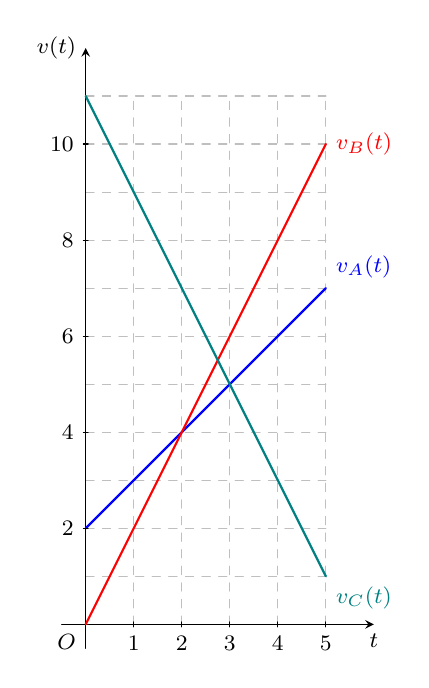
\begin{tikzpicture}[>=stealth,line join=round,line cap=round,font=\footnotesize,scale=.61]
				% Lưới 
				\draw[lightgray, dashed] (0,0) grid (5,11);
				% Vẽ hệ trục tọa độ
				\draw[->] (-0.5,0) -- (6,0) node[below] {$t$};
				\draw[->] (0,-0.5) -- (0,12) node[left] {$v(t)$};
				\node[below left] at (0,0) {$O$};			
				
				% Vẽ đồ thị v_A(t) = t + 2
				\draw[blue, thick, domain=0:5, samples=2] plot (\x, {\x + 2}) node[above right] {$v_A(t)$};
				
				% Vẽ đồ thị v_B(t) = 2t
				\draw[red, thick, domain=0:5, samples=2] plot (\x, {2*\x}) node[right] {$v_B(t)$};
				
				% Vẽ đồ thị v_C(t) = 11 - 2t
				\draw[teal, thick, domain=0:5, samples=2] plot (\x, {11 - 2*\x}) node[below right] {$v_C(t)$};
				
				% Đánh dấu các giá trị trên trục t
				\foreach \x in {1,2,3,4,5} 
				\draw (\x, 0.05) -- (\x, -0.05) node[below] {$\x$};
				
				% Đánh dấu các giá trị trên trục v
				\foreach \y in {2,4,6,8,10} 
				\draw (0.05, \y) -- (-0.05, \y) node[left] {$\y$};
			\end{tikzpicture}
		}				
	}
\end{ex}

%======Câu_4-phần III======%
\begin{ex}%[0D8V2-5]
\immini{Hai bạn An và Bình cùng chơi trò chơi đánh cờ carô trên một bảng ô vuông kích thước $3\times 3$ (gồm $9$ ô trống). Luật chơi quy định An đi trước, mỗi lượt điền một dấu \lq\lq X\rq\rq\ vào một ô trống và Bình đi sau, mỗi lượt điền một dấu \lq\lq O\rq\rq\ vào một ô trống. Trò chơi kết thúc và xác định được người chiến thắng nếu người đó tạo được $3$ dấu của mình nằm liên tiếp nhau trên cùng một hàng ngang, hàng dọc hoặc đường chéo. Hỏi có tất cả bao nhiêu trình tự các nước đi để ván cờ kết thúc chính xác ở nước đi thứ $5$ với An là người giành chiến thắng?
\par\shortans{$1440$}}
	{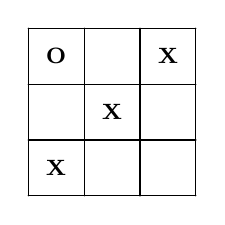
\begin{tikzpicture}[>=stealth,line join=round,line cap=round,font=\footnotesize,scale=.71]
			\draw (0,0) grid (3,3);
			\node at (0.5,2.5) {\textbf{O}};
			\node at (1.5,1.5) {\textbf{X}};
			\node at (2.5,2.5) {\textbf{X}};
			\node at (0.5,0.5) {\textbf{X}};
	\end{tikzpicture}}
\loigiai{
		Ván cờ kết thúc ở nước thứ $5$ nghĩa là An đánh nước thứ $3$ của mình và thắng ngay lập tức.\\
		Khi đó, An có $3$ quân \lq\lq X\rq\rq\ và Bình có $2$ quân \lq\lq O\rq\rq.\\
		Số cách chọn $3$ ô để An thắng (tạo thành hàng ngang, dọc hoặc chéo) là $8$ cách (3 hàng, 3 cột, 2 chéo).\\
		Với mỗi bộ $3$ ô thắng của An, có $3!$ trình tự đánh của An.\\
		Số cách chọn $2$ ô từ $6$ ô còn lại cho Bình là $\mathrm{C}_6^2=15$ cách.\\
		Với mỗi bộ $2$ ô của Bình, có $2!$ trình tự đánh của Bình.\\
		Vậy số trình tự là $8 \cdot 3! \cdot 15 \cdot 2! = 8 \cdot 6 \cdot 15 \cdot 2 = 1440$.
	}
\end{ex}

%======Câu_5-phần III======%
\begin{ex}%[2D1V5-8]
	Một doanh nghiệp sản xuất thiết bị điện tử thông minh có quy trình vận hành và chính sách thuế như sau: Trong mỗi tháng, doanh nghiệp phải chi trả một khoản chi phí cố định $200$ triệu đồng, khoản chi phí này không phụ thuộc vào số lượng sản phẩm sản xuất. Ngoài ra, để hoàn thiện mỗi sản phẩm, doanh nghiệp phải chịu chi phí biến đổi $1$ triệu đồng cho mỗi sản phẩm. Mỗi sản phẩm được bán ra thị trường với giá $3$ triệu đồng một sản phẩm. Nhằm khuyến khích gia tăng quy mô sản xuất, cơ quan quản lý áp dụng chính sách thuế tính theo tổng doanh thu trong tháng, với mức thuế suất giảm dần theo sản lượng. Nếu doanh nghiệp bán dưới $100$ sản phẩm trong tháng, thuế suất là $10\%$ tổng doanh thu. Nếu bán từ $100$ đến dưới $300$ sản phẩm, thuế suất là $8\%$ tổng doanh thu. Nếu bán từ $300$ sản phẩm trở lên, thuế suất là $5\%$ tổng doanh thu. Gọi $x$ là số lượng sản phẩm doanh nghiệp sản xuất và bán ra trong một tháng ($x\in\mathbb{N}^*$). Tìm số sản phẩm tối thiểu để doanh nghiệp bắt đầu có lãi.
\par\shortans{$114$}
\loigiai{
		Tổng chi phí là $C(x)=200+x$ (triệu đồng).\\
		Tổng doanh thu là $R(x)=3x$ (triệu đồng).\\
		Lợi nhuận là $L(x)=R(x)-C(x)-T(x)$, trong đó $T(x)$ là thuế ứng với $x$ số lượng sản phẩm.\\
		Doanh nghiệp có lãi khi $L(x)>0$. Xét các trường hợp sau
		\begin{itemize}
			\item \textbf{Trường hợp 1:} $x<100$.\\
			Ta có $T(x)= 10\% \cdot 3x = 0{,}3x$. Do đó $L(x)=3x-(200+x)-0{,}3x = 1{,}7x-200$.\\
			Khi đó $1{,}7x-200>0 \Rightarrow x>117{,}6$ (Loại vì $x<100$).
			\item \textbf{Trường hợp 2:} $100 \le x < 300$.\\
			Ta có $T(x)= 8\% \cdot 3x = 0{,}24x$. Do đó $L(x)=3x-(200+x)-0{,}24x = 1{,}76x-200$.\\
			Khi đó $1{,}76x-200>0 \Rightarrow x>113{,}63$. Vì $x$ nguyên dương nên $x_{\text{min}}=114$.
			\item \textbf{Trường hợp 3:} $x \ge 300$.\\
			Ta có $T(x)= 5\% \cdot 3x = 0{,}15x$. Do đó $L(x)=3x-(200+x)-0{,}15x = 1{,}85x-200$.\\
			Với $x \ge 300$ thì $L(x)$ luôn dương, nhưng ta tìm số tối thiểu nên giá trị cần tìm nằm ở trường hợp 2.
		\end{itemize}		
		Vậy số sản phẩm tối thiểu là $114$.
	}
\end{ex}

%======Câu_6-phần III======%
\begin{ex}%[1D2H2-7]
	Bé An vừa kết thúc năm học lớp 1. Nghỉ hè, mẹ bé khuyến khích bé An tập viết để chữ viết đẹp và viết được nhanh hơn. Mẹ giao ngày thứ hai này bé luyện viết 1 trang trong quyển luyện viết và cứ thế tăng mỗi ngày thêm một trang. Đến ngày chủ nhật của tuần đó bé An đã viết được tất cả bao nhiêu trang luyện chữ?
	\par\shortans{$28$}
\loigiai{
		Số trang bé An viết mỗi ngày từ thứ Hai đến Chủ nhật lập thành một cấp số cộng với $u_1=1$, công sai $d=1$.\\
		Từ thứ Hai đến Chủ nhật có tất cả 7 ngày, tương ứng với $n=7$.\\
		Số trang viết được ở mỗi ngày lần lượt là: 1, 2, 3, 4, 5, 6, 7.\\
		Tổng số trang bé An viết được là $S_7=1+2+3+4+5+6+7=28$.\\
	}
\end{ex}
 